\chapter{PLANTEAMIENTO DEL PROBLEMA}
\section{Descripción de la Realidad Problemática}

A nivel mundial, la predicción de la demanda de productos perecibles enfrenta desafíos significativos debido a la complejidad de los factores externos, la disponibilidad limitada de datos completos y precisos, la variabilidad en la vida útil de los productos, la naturaleza estática de muchos modelos predictivos, los desafíos logísticos y de distribución, así como los costos asociados con errores en las predicciones. Mejorar la rentabilidad en este contexto requiere el desarrollo de modelos más sofisticados que consideren estos desafíos y una gestión efectiva de la cadena de suministro para minimizar los riesgos financieros asociados con la incertidumbre en la demanda. Por ejemplo, un estudio realizado en China examinó la importancia de la precisión en las predicciones para evitar pérdidas en la industria de alimentos perecibles en el contexto de la rentabilidad empresarial (\cite{foodbank}). Además, en un trabajo llevado a cabo en Estados Unidos, se destacó la influencia de factores externos como las condiciones climáticas y los cambios en los hábitos de consumo en la demanda de productos perecibles, lo cual impacta directamente en la rentabilidad de las empresas. Estas investigaciones reflejan la preocupación global por mejorar la capacidad predictiva en el ámbito de los productos perecibles para optimizar la rentabilidad en un contexto empresarial cada vez más competitivo.

En este contexto, la aplicación de minería de datos y modelos de pronóstico se presenta como una solución estratégica. ``Bajo esta premisa, la utilización de pronósticos en estos productos ayudará a planificar de mejor forma el proceso de abastecimiento, a través de métodos cuantitativos. Para llevar a cabo este estudio se aplica un análisis de autocorrelación a todas las series de tiempo, con el fin de verificar la estacionalidad o aleatoriedad de los productos''. Otro desafío importante es la capacidad de las empresas para aprovechar al máximo los datos disponibles. Muchas empresas peruanas, especialmente las pequeñas y medianas, pueden carecer de la infraestructura y la experiencia necesarias para implementar eficazmente soluciones de análisis de información. Aunque Perú ya cuenta con dos ediciones de la Agenda Digital y ha manifestado un notable interés político en promover el uso de las TIC y el crecimiento de la Sociedad de la Información, los esfuerzos por establecer un marco institucional y una política completa que impulse la transformación digital del país aún no han sido suficientes (\cite{HerediaCEPAL}). Esto puede deberse a limitaciones presupuestarias, falta de talento especializado o simplemente falta de conocimiento sobre las ventajas que pueden ofrecer estas tecnologías. Además, el aspecto regulatorio y de privacidad también es un factor crucial. A medida que las empresas recopilan y analizan grandes cantidades de datos, es fundamental garantizar que lo hagan de manera ética y cumpliendo con las leyes de protección de datos. En Perú, como en muchos otros lugares, la regulación en torno a la privacidad de los datos está en constante evolución, lo que puede plantear desafíos adicionales para las empresas que buscan aprovechar el potencial del análisis.

La decisión de incorporar Machine learning se fundamenta en la necesidad de abordar problemas específicos en el manejo del stock y la toma de decisiones. ``Es por ello que se ha creído conveniente hacer uso de IA, ya que en la empresa existen problemas respecto al stock de productos y esencialmente en la toma de decisiones. Los modelos de pronóstico son un procedimiento matemático que se utiliza para prevenir eventos o desenlaces futuros a través del análisis de patrones'' \cite{MINTARYA202396}. El objetivo es mejorar la precisión de la proyección de ventas futuras, un aspecto crítico en la estrategia empresarial y la toma de decisiones. ``Se han seleccionado diversos  algoritmos de aprendizaje automático, como Random Forest, Regresion lineal, ARIMA y Redes Neuronales entreo otras implementadas en Keras, para su aplicación en datos de ventas del año 2023 al 2024. Estos modelos se compararán en términos de precisión y eficacia en la proyección de ventas''.

En Perú, en el actual escenario de crecimiento económico del 2.3\% entre 2014 y 2023 (\cite{Bancomundial}). Las empresas, incluida Donna S.A.C., han experimentado una expansión significativa en sus operaciones. Este aumento ha llevado consigo la gestión de una cantidad considerable de información, planteando desafíos cruciales en cuanto al procesamiento y análisis preciso de datos en tiempo real. Esta complejidad ha generado una toma de decisiones basada en datos subjetivos, afectando negativamente la planificación estratégica. Específicamente para Donna S.A.C., la gestión del stock de productos y la toma de decisiones relacionadas presentan obstáculos sustanciales. La falta de establecimiento de cantidades óptimas de productos para satisfacer la demanda, así como la identificación de productos más rentables, son problemas evidentes. A pesar de la importancia de la predicción en este entorno dinámico, se observa una marcada escasez de investigaciones dedicadas a la implementación de modelos predictivos y técnicas de minería de datos en este contexto.

Esta aplicación específica de técnicas avanzadas de pronóstico en el ámbito minorista destaca la falta de investigaciones centradas en la predicción en empresas de este sector, evidenciando la urgencia de adoptar enfoques innovadores para mejorar la eficacia de la gestión de inventario y la toma de decisiones estratégicas en Donna S.A.C.

%\medskip
 



%{	\begin{figure}[h]
%		\begin{center}
%			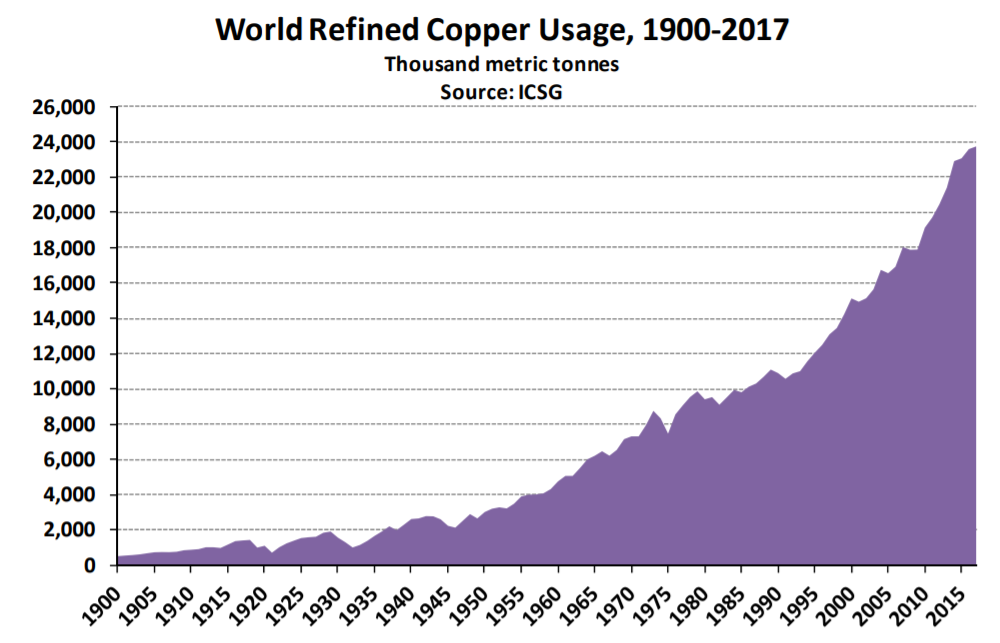
\includegraphics[width=0.8\textwidth]{1/figures/world_refined_copper_usage.png}
%			\caption{Uso del cobre refinado mundial del año 1900 a 2017 (en miles de toneladas). Fuente: \cite{cu_internationalcopper2018}}
%			\label{1:fig}
%		\end{center}
%	\end{figure}
%	}
%	
%	A lo largo de los años, como se observa en la Figura \ref{1:fig}, el uso del cobre refinado (cobre de alta pureza con una concentración de 99.9\%) en el mundo ha tenido un incremento bastante significativo y ello ha conllevado a un aumento en la comercialización de dicho metal. Como consecuencia, este ha contribuido en gran medida para las economías de diversas naciones ya sean países maduros o en vías de desarrollo. El minado, procesamiento, reciclaje y transformación de este metal a varios productos ha creado trabajos y generado riqueza. Estas actividades contribuyen en construir y mantener la infraestructura de un país, y además crea oportunidades de comercio e inversión \parencite{cu_internationalcopper2018}.
%	
%	
%	
%	\begin{figure}[h]
%		\begin{center}
%			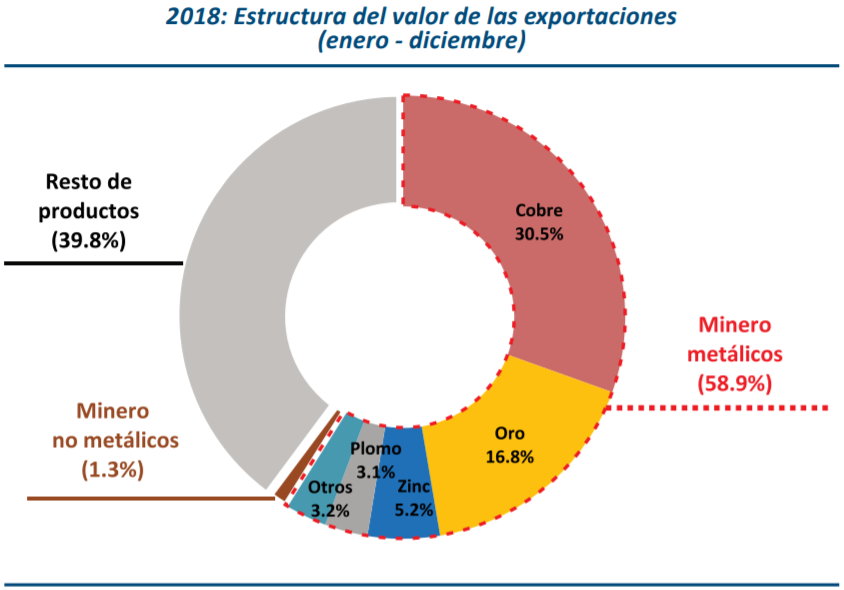
\includegraphics[width=0.8\textwidth]{1/figures/estructura_exportaciones_peru.png}
%			\caption{Estructura del valor de las exportaciones peruanas en el año 2018. Fuente: \cite{cu_ministerioPeru_statsminas}}
%			\label{1:fig2}
%		\end{center}
%	\end{figure}
%	
%	
%	
%	
%	\begin{figure}[h]
%		\begin{center}
%			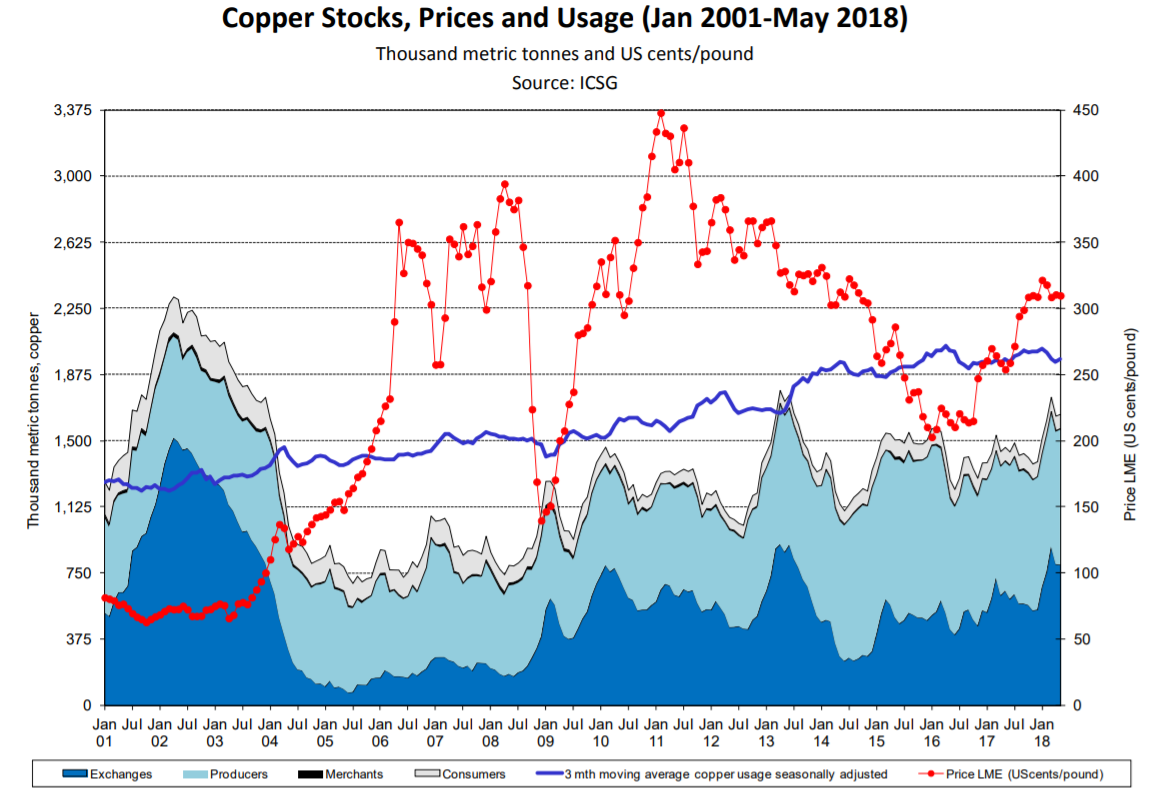
\includegraphics[width=0.8\textwidth]{1/figures/copper_stocks_prices_usage.png}
%			\caption{Precio, stocks y uso del cobre (cantidad en miles de toneladas y precio en centavos por libra). Fuente: \cite{cu_internationalcopper2018}}	
%			\label{1:fig3}
%		\end{center}
%	\end{figure}
%	
%	Estos modelos usados para predecir precios se basan mayormente en estimaciones de la oferta y demanda futura, así como los inventarios de bolsa. Otros consideran la memoria histórica de estas variables, la información de costos futuros de proyectos mineros, o variables financieras. Sin embargo, lo que estos modelos no hacen, es predecir el momento de la caída o alza del precio debido a eventos que no dependen de ninguna de las variables antes mencionadas sino a hechos inesperados globales \citep{cu_lagos2017proyectar}. 
%	
%	
%	\begin{figure}[h]
%		\begin{center}
%			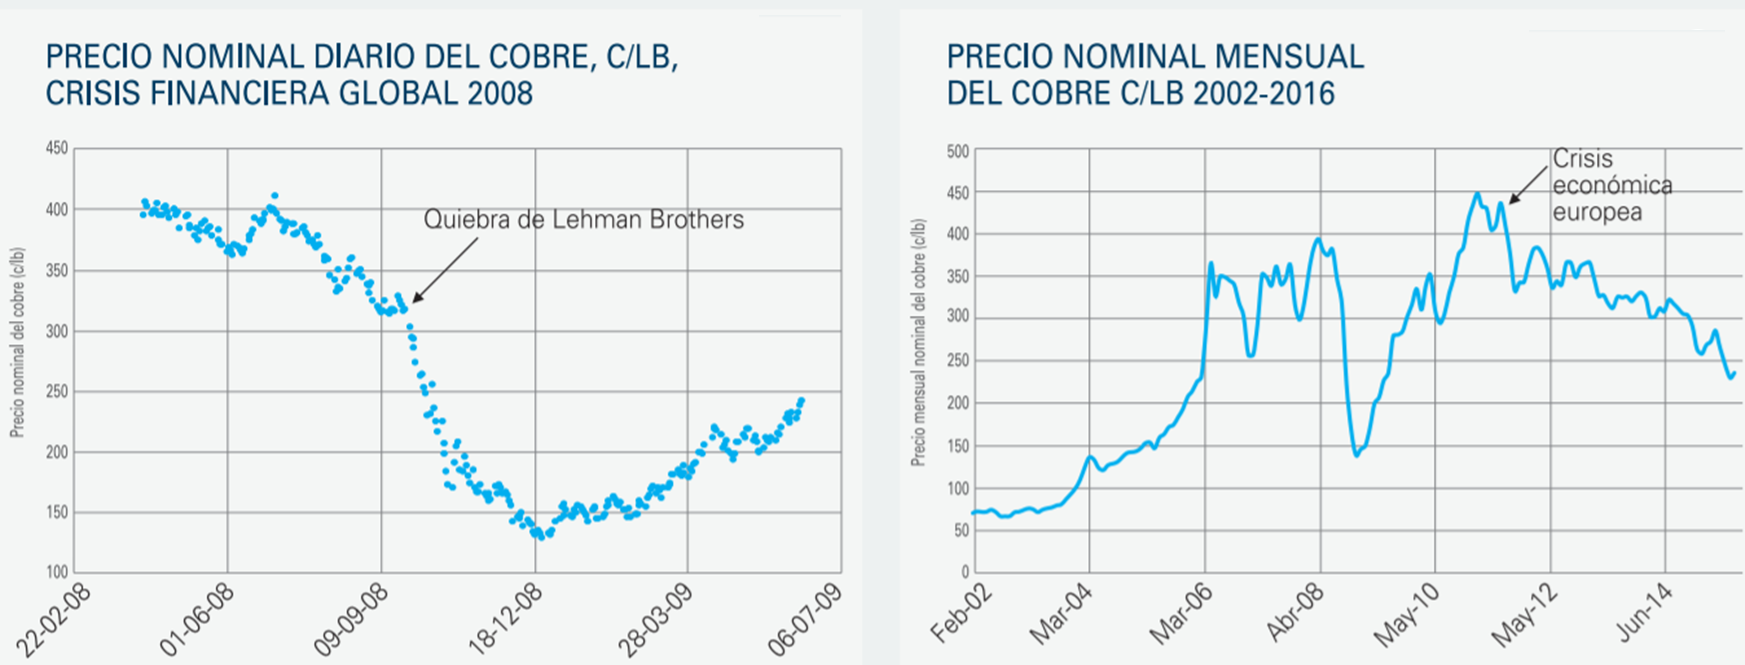
\includegraphics[width=0.8\textwidth]{1/figures/precio_caidas_gustavo_lagos.png}
%			\caption{Precio, stocks y uso del cobre (cantidad en miles de toneladas y precio en centavos por libra). Fuente: \cite{cu_lagos2017proyectar}}
%			\label{1:fig4}
%		\end{center}
%	\end{figure} 




\section{Formulación del Problema}

%Para lefecto \parencite{ot_marti2018manual}. 
%
%
%Una vez elaborado el diagrama (véase Anexo 1), 

\subsection{Problema General}
\newcommand{\ProblemaGeneral}{
	¿Como la implementación de un modelo predictivo de la demanda de productos perecibles beneficiará la toma de decisiones en el proceso del pedido a los proveedores en la empresa Donna SAC?  
}
\ProblemaGeneral
\subsection{Problemas Espec\'{i}ficos}
\newcommand{\Pbone}{
¿Cómo pueden los modelos de predicción de demanda contribuir a una planificación de existencias de productos?
}
\newcommand{\Pbtwo}{
¿Qué técnicas de preprocesamiento de datos son más efectivas para mejorar la precisión de los modelos de predicción de demanda en productos perecibles?
}
\newcommand{\Pbthree}{
¿Cuál es la influencia de las variables de la demanda para predecir productos perecibles y como pueden ajustarse en función al modelo?
}
\newcommand{\Pbfour}{
¿Cuál es la función de los modelos avanzados de Forecasting de la demanda y cómo se comparan con otros métodos de aprendizaje automático en cuanto a precisión y aplicabilidad?
}
%\newcommand{\Pbfive}{
%A
%}

\begin{itemize}
	\item \Pbone
	\item \Pbtwo
	\item \Pbthree
	\item \Pbfour
%	\item \Pbfive
\end{itemize}

\section{Objetivos de la Investigación}
%Para la formulación de los objetivos de la presente investigación se elaboró un «árbol de objetivos» (véase Anexo 2) 
\subsection{Objetivo General}
\newcommand{\ObjetivoGeneral}{
Implementar un modelo predictivo de la demanda de productos perecibles que beneficie la toma de decisiones en el proceso del pedido a los proveedores en la empresa Donna SAC.
}
\ObjetivoGeneral
\subsection{Objetivos Espec\'{i}ficos}
\newcommand{\Objone}{
Determinar cómo los modelos de predicción de demanda pueden contribuir a optimizar la planificación de existencias de productos.
}
\newcommand{\Objtwo}{
Determinar las técnicas de preprocesamiento de datos más efectivas para mejorar la precisión de los modelos de predicción de demanda en productos perecibles. 
}
\newcommand{\Objthree}{
Determinar que variables de la demanda influyen en predecir productos perecibles. 
}
\newcommand{\Objfour}{
Evaluar la eficacia de los modelos avanzados de Forecasting en la predicción de la demanda en una tienda, comparándolos con otros métodos de aprendizaje automático en términos de precisión y aplicabilidad
}
%\newcommand{\Objfive}{
%ghhhg
%}

\begin{itemize}
	\item {\Objone}
	\item {\Objtwo}
	\item {\Objthree}
	\item {\Objfour}
%	\item {\Objfive}
\end{itemize}

\section{Justificación de la Investigación}

\subsection{Teórica}
Se justifica teóricamente primeramente porque las técnicas de aprendizaje automático pueden analizar conjuntos de datos más grandes con mayor eficiencia y precisión que los métodos convencionales, lo que posibilita proporcionar un entendimiento aún más profundo de los patrones y tendencias. Este estudio tiene como propósito aportar nuevos conocimientos en el big data de datos mediante la implementación de técnicas avanzadas de forecasting de series de tiempo. El resultado satisfactorio de este enfoque está destinado a ser utilizado en la gestión precisa de la demanda de productos en el sector minorista, contribuyendo así a la optimización de procesos y la toma de decisiones estratégicas. En conjunto, se busca la eficacia global de la gestión de inventario en el ámbito de la minería de datos. 

\subsection{Práctica}
Esta investigación surge en respuesta a la imperante necesidad de optimizar el aprovechamiento de la valiosa base de datos de nuestra empresa. Nos proponemos no solo hacer uso de los datos históricos disponibles, sino también desarrollar e implementar un modelo predictivo eficiente. El propósito primordial es transformar estos pronósticos en herramientas esenciales para respaldar decisiones estratégicas informadas en la gestión de abastecimiento para nuestras tiendas minoristas. Resaltando esta justificación práctica, buscamos mejorar el desempeño y la eficacia de las operaciones mediante una gestión avanzada de la demanda, lo que a su vez impactará positivamente en la satisfacción del cliente, la optimización de inventarios y la rentabilidad general de la empresa.

\subsection{Metodológica}. 
 El principal problema que ayudará a resolver esta investigación es optimizar la precisión de la predicción de la demanda en las tiendas minoristas. Para ello, se implementará la técnica de forecasting aplicada a las series temporales, buscando obtener la mayor precisión posible en las predicciones de demanda. Este enfoque permitirá una gestión más eficaz del inventario y respaldará decisiones estratégicas basadas en datos predictivos más precisos y actualizados. \\
 La metodología incluirá:
 
 \newcommand{\Mone}{
 	Recopilación de datos históricos de ventas de productos perecibles.}
 \newcommand{\Mtwo}{
 	Identificación y recopilación de variables externas relevantes que puedan influir en la demanda (por ejemplo, eventos especiales, condiciones climáticas, tendencias de mercado). 
 }
 \newcommand{\Mthree}{
 	Selección y aplicación de técnicas de modelado predictivo, como regresión lineal, series temporales, o técnicas más avanzadas como modelos de redes neuronales o machine learning. 
 }
 \newcommand{\Mfour}{
 	Validación del modelo utilizando técnicas como la validación cruzada y la comparación de los resultados predichos con los datos reales de ventas.
 	}
 \newcommand{\Mfive}{
 	Implementación del modelo en un entorno empresarial y evaluación de su impacto en la rentabilidad.
 	}
 
 \begin{itemize}
 	\item {\Mone}
 	\item {\Mtwo}
 	\item {\Mthree}
 	\item {\Mfour}
 	\item {\Mfive}
 \end{itemize}

\section{Delimitación del Estudio}

\subsection{Espacial}
Se realizará en la empresa Donna S.A.C. ubicada en el distrito de Breña, Provincia y Departamento de Lima. Teniendo como giro principal la venta de productos de supermercado. 

\subsection{Temporal}
Se llevará a cabo en la empresa Donna S.A.C. mediante el análisis de los datos mensuales obtenidos desde el año 2023 al 2024, los cuales se obtendrán a partir de la data registrada por la empresa y proporcionados por el personal encargado del manejo de datos. 

\subsection{Conceptual}
La presente, realizada en la empresa Donna S.A.C., se enfoca en la implementación de un modelo de Series de tiempo basado en algoritmos de aprendizaje automático. Este enfoque nos ayudará a realizar predicciones en la empresa, y la implementación se llevará a cabo utilizando herramientas básicas de producción. Se establecerán relaciones entre las diversas áreas presentes dentro de la empresa. Se evaluarán los beneficios que atraerá dicha implementación y se buscarán maneras de continuar mejorando el proceso.

\section{Hipótesis}

\subsection{Hipótesis General}
\newcommand{\HipotesisGeneral}{
La implementación de un modelo predictivo de la demanda de productos perecibles beneficiara en la toma de decisiones en el proceso de pedido a los proveedores en la empresa Donna SAC.
}
\HipotesisGeneral
\subsection{Hipótesis Específicas}
\newcommand{\Hone}{
El uso de modelos de predicción de demanda mejora la planificación de existencias de productos asegurando la disponibilidad adecuada.
}
\newcommand{\Htwo}{
Las técnicas de procesamiento de datos como la normalización de datos, el tratamiento de valores atípicos y la selección de características relevantes, serán más efectivas para mejorar la precisión de los modelos de predicción de demanda en productos perecibles  
}
\newcommand{\Hthree}{
 Las variables escogidas de la demanda tienen influencia significativa en el modelo.
}
\newcommand{\Hfour}{
Los modelos avanzados de Forecasting proporcionan una mayor precisión y aplicabilidad en la predicción de la demanda en un entorno de tienda, en comparación con otros métodos de aprendizaje automático
}
%\newcommand{\Hfive}{
%	xws
%}
\begin{itemize}
	\item \Hone
	\item \Htwo
	\item \Hthree
	\item \Hfour
%	\item \Hfive
\end{itemize}

\subsection{Matriz de Consistencia}
A continuación se presenta la matriz de consistencia elaborada para la presente investigación (véase Anexo \ref{1:table}).

